% 02_background.tex  - concise (≤ 3 pp.), details in Appendix A
% ------------------------------------------------------------------
\section{Theoretical Background \& Related Work}
\label{sec:background}

\paragraph{Notation.} We denote \(T_p\) and \(T_f\) as the numbers of observed and predicted timesteps, respectively. Following UniTraj conventions~\cite{unitrajFeng2024}, agent trajectories are represented as \(\boldsymbol{X}_d \in \R^{N_{\max} \times T_p \times F_{ap}}\) and map polylines as \(\boldsymbol{X}_s \in \R^{K_{\max} \times L \times F_{map}}\), where \(N_{\max}\) is the maximum number of agents, \(K_{\max}\) is the maximum number of map polylines, \(L\) is the points per polyline, and \(F_{ap}, F_{map}\) are the respective feature dimensions. Ground truth trajectories for the center agent are denoted \(\boldsymbol{y}_c \in \R^{T_f \times 4}\). For rasterized approaches, BEV representations use \(H \times W\) spatial resolution with \(F_d, F_s\) channel dimensions for dynamic and static inputs, respectively. Transformer models employ \(M\) output modes, \(K_s\) sampling points per deformable attention query, and \(N_h\) attention heads. Feature pyramid networks utilize \(L_{\text{FPN}}\) levels indexed by \(\ell \in \{0,\dots,L_{\text{FPN}}-1\}\), with feature maps \(C_\ell \times H_\ell \times W_\ell\) at each level. A comprehensive symbol table is provided in Appendix~\ref{app:notation}.

%--------------------------------------------------------------------

\subsection{Scene Representation Paradigms}
\label{ssec:scene_repr}
% TODO: Introduction into what is generally meant by a scene representation in the context of trajectory prediction, and why it is important.
% Highlight, why accurate scene representations are crucial for motion forecasting in the borader context of autonomous driving.
% TODO: refer to the two figures below in the description of each paradigm!

Scene representations translate outputs of the perception stage into a tensor that subsequent neural modules can exploit. Desirable properties include:
\begin{enumerate}[label=\roman*)]
    \item high geometric fidelity
    \item invariance to global transformations (translation, rotation, time-shift) \( SE(2) \rtimes \R \)
    \item information density, ensuring that representations encode all relevant properties of the scene without unnecessary redundancy
    \item suitability for efficiently modeling spatio-temporal, kinematic, semantic, and topological relationships between scene elements
    \item computational re-use across frames~\cite{qcnetZhou2023,lmformerYadav2025}.
\end{enumerate}
The choice of scene representation fundamentally affects how effectively the predictor can capture essential relationships and dynamics in complex traffic scenarios, and hence it's capacity to produce accurate and diverse motion forecasts. The \emph{rasterized} and \emph{vectorized} paradigms represent the two main approaches to scene representation in trajectory prediction, as illustrated in~\autoref{fig:scene_representations}.

\begin{figure}[H]
\centering
\begin{subfigure}[t]{0.35\textwidth}
    \centering
    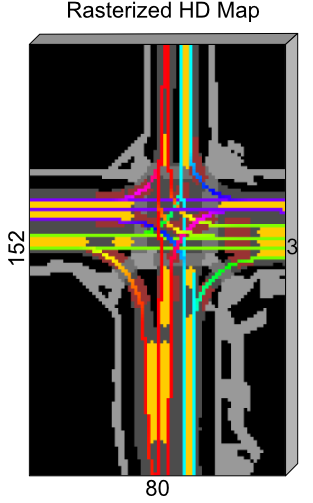
\includegraphics[width=\textwidth]{figures/caspnet-bev-repr.png}
    \caption{Rasterized BEV encoding}
    \label{fig:rasterized}
\end{subfigure}
\hfill
\begin{subfigure}[t]{0.37\textwidth}
    \centering
    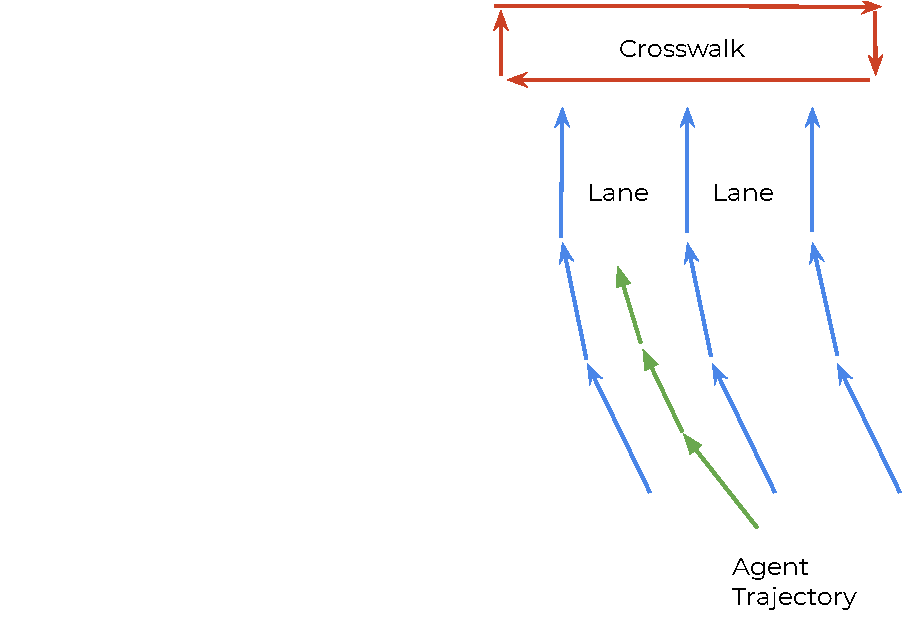
\includegraphics[width=\textwidth]{figures/vectornet-2020-vector-repr.pdf}
    \caption{Vectorized polyline preservation}
    \label{fig:vectorized}
\end{subfigure}
\caption{Scene representation paradigms in trajectory prediction: (a) rasterized approaches stack agent trajectories and HD maps into BEV images~\cite{caspnetSchäfer2022}, (b) vectorized methods preserve geometric polylines~\cite{gao2020vectornet}.}
\label{fig:scene_representations}
\end{figure}

% TODO: use \begin{description}
%   \item[]
% \end{description} instead of textbf{} to introduce the two paradigms

\begin{description}
\item[Raster grids.] Early systems stack past agent masks and HD-map layers into \( F \)-dimensional BEV (Bird's Eye View) images, leveraging convolutional backbones to capture spatial relationships while keeping runtime independent of the number of agents~\cite{cui2019multimodal,chai2019multipath}. Specifically, these approaches construct: (i) a BEV stack of past agent trajectories \( \mathbf{I}_d\in\R^{T_p\times H\times W\times F_d} \) and (ii) a static HD-map raster \( \mathbf{I}_s\in\R^{H\times W\times F_s} \).\\
The CASPNet family of motion forecasting models, consisting of the original CASPNet~\cite{caspnetSchäfer2022}, which utilizes a fully convolutional architecture, CASPNet++~\cite{caspnetppSchäfer2023}, and the CASPFormer~\cite{caspformerYadav2024}, exemplifies interesting architectural choices within this paradigm and will be discussed in greater detail in~\autoref{ssec:caspnet}.\\
However, rasterized approaches suffer from limited geometric fidelity and redundant pixel information due to grid-based discretization of scene elements' geometric and kinematic properties~\cite{lmformerYadav2025}. Additionally, respecting agent identities is infeasible as it would require separate channels per agent, introducing further redundancy; CASPNet++~\cite{caspnetppSchäfer2023} addressed this using single BEV per agent. Furthermore, rasterized approaches allow only shared coordinate systems, which is suboptimal for leveraging geometric isomorphisms~\cite{qcnetZhou2023}. % TODO: it is infeasible to respect the identities of agents as this would require a separate channel or set of channels for each agent throughout the entire architecture, which would introduce even more redundancy in terms of pixel information. However, respecting identities is crucial for true multi-agent motion forecasting, the aforementioned approach of using a single BEV per agent was used in \cite{caspnetppSchäfer2023}. Additionally, rasterized approaches allow only a shared coordinate system, which is suboptimal in terms of leverageable geometric isomorphisms.

\item[Vector representations.] Later work encodes agents and lanes as vectorized geometric primitives such as polylines, enabling graph (LaneGCN~\cite{liang2020learning}, VectorNet~\cite{VectorNet2020}) or transformer based (QCNet~\cite{qcnetZhou2023}, QCNeXt~\cite{qcnextZhou2023}, LMFormer~\cite{lmformerYadav2025}) approaches with higher geometric fidelity but runtime that grows with scene complexity. These representations are more compact, preserve higher geometric fidelity, and enable explicit modeling of complex spatio-temporal and social relationships between scene elements. Lane information uses two main representations:
\begin{itemize}
  \item \textbf{Point-based}: Each polyline \(L_p^i = [P_1^i, P_2^i, \ldots, P_K^i]\) with \(K\) control points \(P_k^i\)~\cite{VectorNet2020, zhou2022hivt}.
  \item \textbf{Segment-based}: Converts to \(L_v^i = [V_1^i, V_2^i, \ldots, V_{K-1}^i]\) where \(V_{k}^i = [P_k^i, P_{k+1}^i]\) stores lane segment vectors. This explicitly encodes road curvature~\cite{liang2020learning,zhou2022hivt,qcnetZhou2023}.
\end{itemize}
Agent trajectories use analogous representations:
\begin{itemize}
  \item \textbf{Trajectory points}: \(\mathcal{T}_{in}^a = [P_1^a, P_2^a, \ldots, P_T^a]\) with global positions \(P_t^a\).
  \item \textbf{Motion vectors}: \(M_t^a = [P_{2}^a - P_{1}^a, \ldots, P_{T}^a - P_{T-1}^a]\) derived from trajectories, representing the displacement between timesteps~\cite{lmformerYadav2025}.
\end{itemize}
Vectorized approaches employ either \emph{agent-centric} coordinate systems (all scene elements normalized to a single ego-centric frame) or \emph{query-centric} paradigms. The choice fundamentally affects computational efficiency, invariance properties, and multi-agent reasoning capabilities, with query-centric approaches offering significant advantages for streaming applications and parallel multi-agent prediction~\cite{qcnetZhou2023}. % TODO: introduce the Vector Based Representation by saying that they are more compact and preserve more geometric fidelity, they are more appropriate for the use in transformer or graph based approaches and allow to model complex spatio-temporal and social relationships between scene elements more explicitly. % TODO: elaborate more closely what agent-centric means: i.e. a single ego-centric coordinate system for all agents.
\end{description}
%% FINISHED UNTIL HERE %%
UniTraj~\cite{unitrajFeng2024} employs a vectorized and agent-centric representation, representing both agent trajectories as vertex lists and map polylines as uniformly sampled list of vertices.

% This so-called \emph{query-centric} approach will be discussed in greater detail in~\autoref{ssec:qc_paradigm}. CASPNet embodies the \emph{raster} philosophy; CASPFormer adopts a hybrid strategy—retaining a CNN backbone for perception compatibility, but switching to a vectorized transformer decoder for output precision.

%<unstructured-collection-of-information-to-include>
% <include:1>\cite{lmformerYadav2025} into Local frame construction
% TODO: define how each local coodinate frame is defined:
% agents: motion vector's start position as its origin, x axis is instantaneous direction of travel
% map polylines: very lane segment is characterized by its start and end positions in global coordinates. The query-centric coordinate frame for a lane segment is set as follows: we designate the segment's start position as its origin and align the segment's vector direction with its x-axis. As a result, the only feature preserved in this query-centric coordinate frame is the segment's length, which we use as its sole feature in the query-centric embedding generation.
% BOTH of these conventions stem from \cite{lmformerYadav2025}
% </include:1>
% <include:2> in Agent-centric vs. query-centric comparison
% Parallel decoding Usually one-agent-at-a-time for agent centric. Multi-agent parallel: same invariant scene tensor is shared by all target agents for query-centric.
% Latent scene representations are \( SE(2) \rtimes \R \) invariant (What about the impact of the relative descriptors?).
% Memory reuse Agent-Centric:% None → recompute full BEV / agent tokens each step. QC: Cache & reuse: when the window slides, the T-1 overlapping steps' embeddings are identical and can be reused. This makes the implementation in \cite{qcnetZhou2023} efficient in terms of its time complexity but it comes at a hughe memory cost, eg The training process consumes ~160G GPU memory.
% </nclude:2>
% 	1.	Local spacetime frame construction
% <include:1>
% •	Each agent state (p^t_i,\theta^t_i,v^t_i) and each map polygon has its own 3-DOF coordinate frame: origin = current position, x-axis = heading, time axis = current step.
% </include:1>
% 	4.	QC allows for Factorised attention with query-centric keys/values. What are the advantages.
	% •	Three axes: Temporal, Agent-Map, Social (Agent-Agent).
	% •	Because queries/keys include relative embeddings, all outputs remain invariant → can be cached. (Page 3-4) _Query-Centric_Trajectory_Prediction_CVPR_2023_paper-2.pdf](file-service://file-MYr4iwPvX6YAGHzdpzXMma)

% \subsubsection*{The Agent-Centric Paradigm: Progress and Limitations}

% \textbf{Agent-centric normalization:} To attain translation and rotation invariance for a target agent, this scheme re-centers and rotates the entire scene so that the reference agent sits at the origin facing the positive $x$-axis. Although this stabilizes coordinate scales and simplifies learning for that agent, privileging one agent breaks permutation symmetry among multiple agents and demands redundant re-normalization and re-encoding each time the prediction target or time window changes, resulting in substantial computational overhead in streaming and multi-agent settings.

% To address the shortcomings of global encoding, the agent-centric paradigm normalizes all scene elements relative to a designated reference agent—typically the prediction target. By placing the reference agent at the origin and aligning its heading with the positive $x$-axis (see Equation~\ref{eq:agent_centric_transform}), agent-centric encoding offers:
% \begin{itemize}
%     \item \textbf{Translation Invariance:} Scene layouts become independent of their absolute location.
%     \item \textbf{Rotation Invariance:} Aligning the agent's heading simplifies learning of common maneuvers.
%     \item \textbf{Consistent Scale:} Bounded coordinate values improve training stability. In query centric encodigngs the range of possible values is more strongly bounded.
%     \item \textbf{Ego-View:} Mirrors the vehicle's own perspective (all vehicles live in fibers that are quite similar to each other), hence the same features are to be expected for all agents independent of their position. This dramatically shrinks the global manifold of possible scene encodings, making it easier for the model to learn efficient representations through *strong inductive biases* % TODO: how is this redundant from the first two points (translation and rotation invariance)
% \end{itemize} % TODO: mention the symmetries only briefly here and add a new \begin{describe} subsequently $[isomorphisms] to discuss the symmetries in more detail.
% <include:3> shortcomings of agent-centric encoding
% Despite these advantages, agent-centric encoding introduces new challenges:
% \begin{itemize}
%     \item \textbf{Computational Redundancy:} Every change in the prediction target or sliding time window requires re-normalizing and re-encoding the entire scene.
%     \item \textbf{Broken Permutation Symmetry:} Privileging one agent as origin disrupts the natural symmetry among multiple agents, hindering true joint prediction.
%     \item \textbf{Temporal Inconsistency:} Streaming applications incur unnecessary reprocessing of static map elements as the reference frame shifts.
%     \item \textbf{Multi-Agent Inefficiency:} Parallel prediction for multiple agents multiplies encoding costs linearly with the number of agents.
% \end{itemize}
% </include:3> shortcomings of agent-centric encoding

% <include:2> in Agent-centric vs. query-centric comparison
% \begin{itemize}
%     \item \textbf{Efficient reuse:} Encodings are independent of prediction target and can be shared across agents and time steps.
%     \item \textbf{Permutation symmetry:} No agent is privileged; all elements are represented equally.
%     \item \textbf{Multi-agent and streaming:} The same scene encoding can be used for parallel prediction of all agents and for streaming updates.
%     \item \textbf{Joint prediction capability:} Unlike marginal prediction approaches, query-centric models can effectively capture future social interactions among agents.
% \end{itemize}
% </include:2>

% %$[isomorphisms]
% <include:4> in Symmetry group actions -> rename A Geometric Perspective on Scene Representations
% here we need to cite~\cite{bronstein2021geometric}
% \begin{itemize}
%     \item \textbf{Permutation symmetry:} The set of agents and map elements is unordered. The model should be equivariant to permutations of the input.
%     \item \textbf{$\SE(2)$ symmetry:} The laws of physics are invariant under translation and rotation. The model should be equivariant to global $\SE(2)$ transformations.
%     \item \textbf{Temporal symmetry:} The encoding should be invariant to shifts in the time origin (for streaming).
% \end{itemize}
% we want to use this perspective of fiber bundels to explain the symmetries - i.e. the sub manifold of all the agents (where spatial and kinematic properties are represented) are quite similar - hence smaller, hence easier to learn. This is the key inductive bias of the query-centric paradigm, which is not present in the agent-centric paradigm. Same goes for the static map elements.
% And the part of the part of the latent scene representation that encodes the relative spatio-temporal relationships between scene elements is in total much smaller and hence also doesn't require as much representative capacity in the model.
% </include:4> Symmetry group actions -> rename A Geometric Perspective on Scene Representations



% The use of \emph{query-centric} scene encodings~\cite{qcnetZhou2023} represents a paradigm shift in trajectory prediction for autonomous driving, fundamentally altering how the spatio-temporal attributes of both static (agents) and dynamic (map polylines) scene elements are represented. <include:introduction>The query-centric paradigm is grounded in the concept of relative spacetime manifolds, drawing inspiration from Einstein's theory of relativity, where the coordinates of scene elements are not expressed in a \emph{global} or \emph{agent-centric} coordinate system</include:introduction>, but rather in \emph{local} frames defined by each element itself. This approach introduces various symmetries, that can be explored through the lens of differential geometry and geometric deep learning~\cite{bronstein2021geometric}, allowing for the design of models leveraging these inductive biases, resulting in more robust and efficient model architectures. This chapter outlines the limitations of traditional agent-centric encoding schemes and provides a comprehensive overview of the query-centric paradigm, including its mathematical foundations, encoding strategies, and architectural innovations.


% QCNet generalizes vector-based encoders by abandoning a single ego-centric grid in favor of local `fibers' for every map polygon or agent-state, yielding strict roto-translation and temporal invariance while enabling streaming-time reuse~\cite{qcnetZhou2023}. Each map polygon and each agent \emph{state} owns a local spacetime frame \((p,\theta,t)\) (Fig.~\ref{fig:polar-frames-three}). All geometry is expressed in these frames; relative descriptors \([\lvert\lvert p_j-p_i\rvert\rvert_2,\;\Delta\theta_{\text{dir}},\;\Delta\theta_{\text{ori}},\;\Delta t]\) are Fourier-MLP embedded and concatenated to keys/values in factorised attention. Consequently the scene tensor is \textbf{roto-translation \& time invariant}, can be \textbf{cached across sliding windows}, and is \textbf{shared by every target agent}, lowering online complexity from \(O(AT^2)\) to \(O(AT)\)~\cite{qcnetZhou2023}.
% \begin{figure}[ht]
% \centering
% \begin{tikzpicture}[scale=1.2]
%   % Global Cartesian axes
%   \draw[thick,->] (0,0) -- (2,0) node[anchor=north west]{$X_{global}$};
%   \draw[thick,->] (0,0) -- (0,2) node[anchor=south east]{$Y_{global}$};

%   % Global positions of elements
%   \coordinate (e1) at (3,1);
%   \coordinate (e2) at (5,3);
%   \coordinate (e3) at (1,4);

%   % Local origins (fibers) marked as filled dots
%   \draw[blue,fill=white]  (e1) circle(1.5pt) node[below left] {$\hat e_1$};
%   \draw[red,fill=white]   (e2) circle(1.5pt) node[above right] {$\hat e_2$};
%   \draw[green,fill=white] (e3) circle(1.5pt) node[above] {$\hat e_3$};

%   % Local reference frames (Cartesian axes) at each origin
%   \draw[blue,thin,->]  (e1) -- ++(10:0.8)  node[anchor=south] {};
%   \draw[blue,thin,->]  (e1) -- ++(100:0.8) node[anchor=west] {};

%   \draw[red,thin,->]   (e2) -- ++(45:0.8)  node[anchor=south west] {};
%   \draw[red,thin,->]   (e2) -- ++(135:0.8) node[anchor=north] {};

%   \draw[green,thin,->] (e3) -- ++(-30:0.8) node[anchor=east] {};
%   \draw[green,thin,->] (e3) -- ++(60:0.8)  node[anchor=west] {};


%   % Local motion vectors in polar form with varying length and rotation
%   \draw[blue,->,line width=1pt]  (e1) -- ++( 30:1.0) node[anchor=south east] {$(r_1,\theta_1)$};
%   \draw[red,->,line width=1pt]   (e2) -- ++(120:0.8) node[anchor=south west] {$(r_2,\theta_2)$};
%   \draw[green,->,line width=1pt] (e3) -- ++(-45:1.2) node[anchor=north east] {$(r_3,\theta_3)$};

%   % Relative transforms between elements
%   \draw[purple,dotted,->,thick] (e1) -- (e2) node[midway,above] {$T_{12}$};
%   \draw[orange,dotted,->,thick] (e2) -- (e3) node[midway,right] {$T_{23}$};
%   \draw[brown,dotted,->,thick]  (e3) -- (e1) node[midway,left] {$T_{31}$};
% \end{tikzpicture}
% \caption{Query-centric layout with global Cartesian axes, annotated motion vectors \((r_i,\theta_i)\) for each element \(\hat e_1,\hat e_2,\hat e_3\), and relative transforms \(T_{12}\), \(T_{23}\), \(T_{31}\). Each local origin (fiber) is shown as a filled dot.}
% \label{fig:polar-frames-three}
% \end{figure}


% In summary, the query-centric paradigm provides a principled, symmetry-respecting, and efficient foundation for trajectory forecasting. The combination of local polar encodings and relative descriptors yields a flexible and lossless representation, underpinning the success of recent state-of-the-art models. This approach has fundamentally changed how the community thinks about scene representation for autonomous driving, moving from agent-centric to truly democratic, multi-agent reasoning systems.
%</unstructured-collection-of-information-to-include>
%
\subsubsection{The Query-Centric Paradigm}
\label{ssec:qc_paradigm}

\paragraph{The short-comings of agent-centric approaches.}

While the agent-centric paradigm is a conceptually simple solution that aligns well with the historical focus on single-agent prediction, where the entire scene is expressed in a global frame centered on the ego vehicle, it is not well-suited for the emerging task of \emph{multi-agent} motion forecasting as it yields roto-translation and time-invariance for only the center agent~\cite{lmformerYadav2025}. \\
Furthermore, this approach becomes computationally infeasible when utilized within the framework of \emph{factorized attention}. While typical encoding strategies, such as those employed in the CASPNet family, squeeze the entire temporal dimension, and subsequently apply agent-map and agent-agent fusion on this time-invariant representation, factorized attention maintains separate spatio-temporal latent representation of all entities in the scene, allowing the model to capture more complex spatio-temporal relationships, such as the interactions between mutliple agents over the course of multiple timesteps. However, this implies cubic complexity for each fusion step:
\begin{equation}
  \begin{aligned}
    \text{Temporal:}      & \quad \mathcal{O}\!\bigl(N_{\max}T^{2}\bigr) \\
    \text{Agent\(\leftrightarrow\)Map Fusion @ $t$:}    & \quad \mathcal{O}\!\bigl(N_{\max}T K\bigr)  \\
    \text{Agent\(\leftrightarrow\)Agent Fusion @ $t$:}  & \quad \mathcal{O}\!\bigl(N_{\max}^{2}T\bigr)
  \end{aligned}
\end{equation}
where \(N_{\max}\) is the maximum number of agents, \(T = T_p + T_f\) the number of total timesteps, and \(K\) is the number of map polylines. This cubic complexity arises from the need to compute pairwise interactions between all agents and map elements at each timestep, leading to significant computational overhead in dense traffic scenarios. \\

\paragraph{Query-centric encodings}
The query-centric paradigm aims to maintain the representational capacity of factorized attention, while reducing the inference latency. The most significant downside of the agent-centric paradigm in this context is that it requires the entire scene to be re-encoded at every timestep, as the location and heading of the target agent change. This means that the model must recompute the entire scene representation for each target agent at \emph{each timestep}, leading to a significant incr6ase in computational complexity and latency, especially in scenarios with many agents and long observation windows~\cite{qcnetZhou2023}.\\

\begin{figure}[H]
  \centering
  \label{fig:qc_reference_frame}
  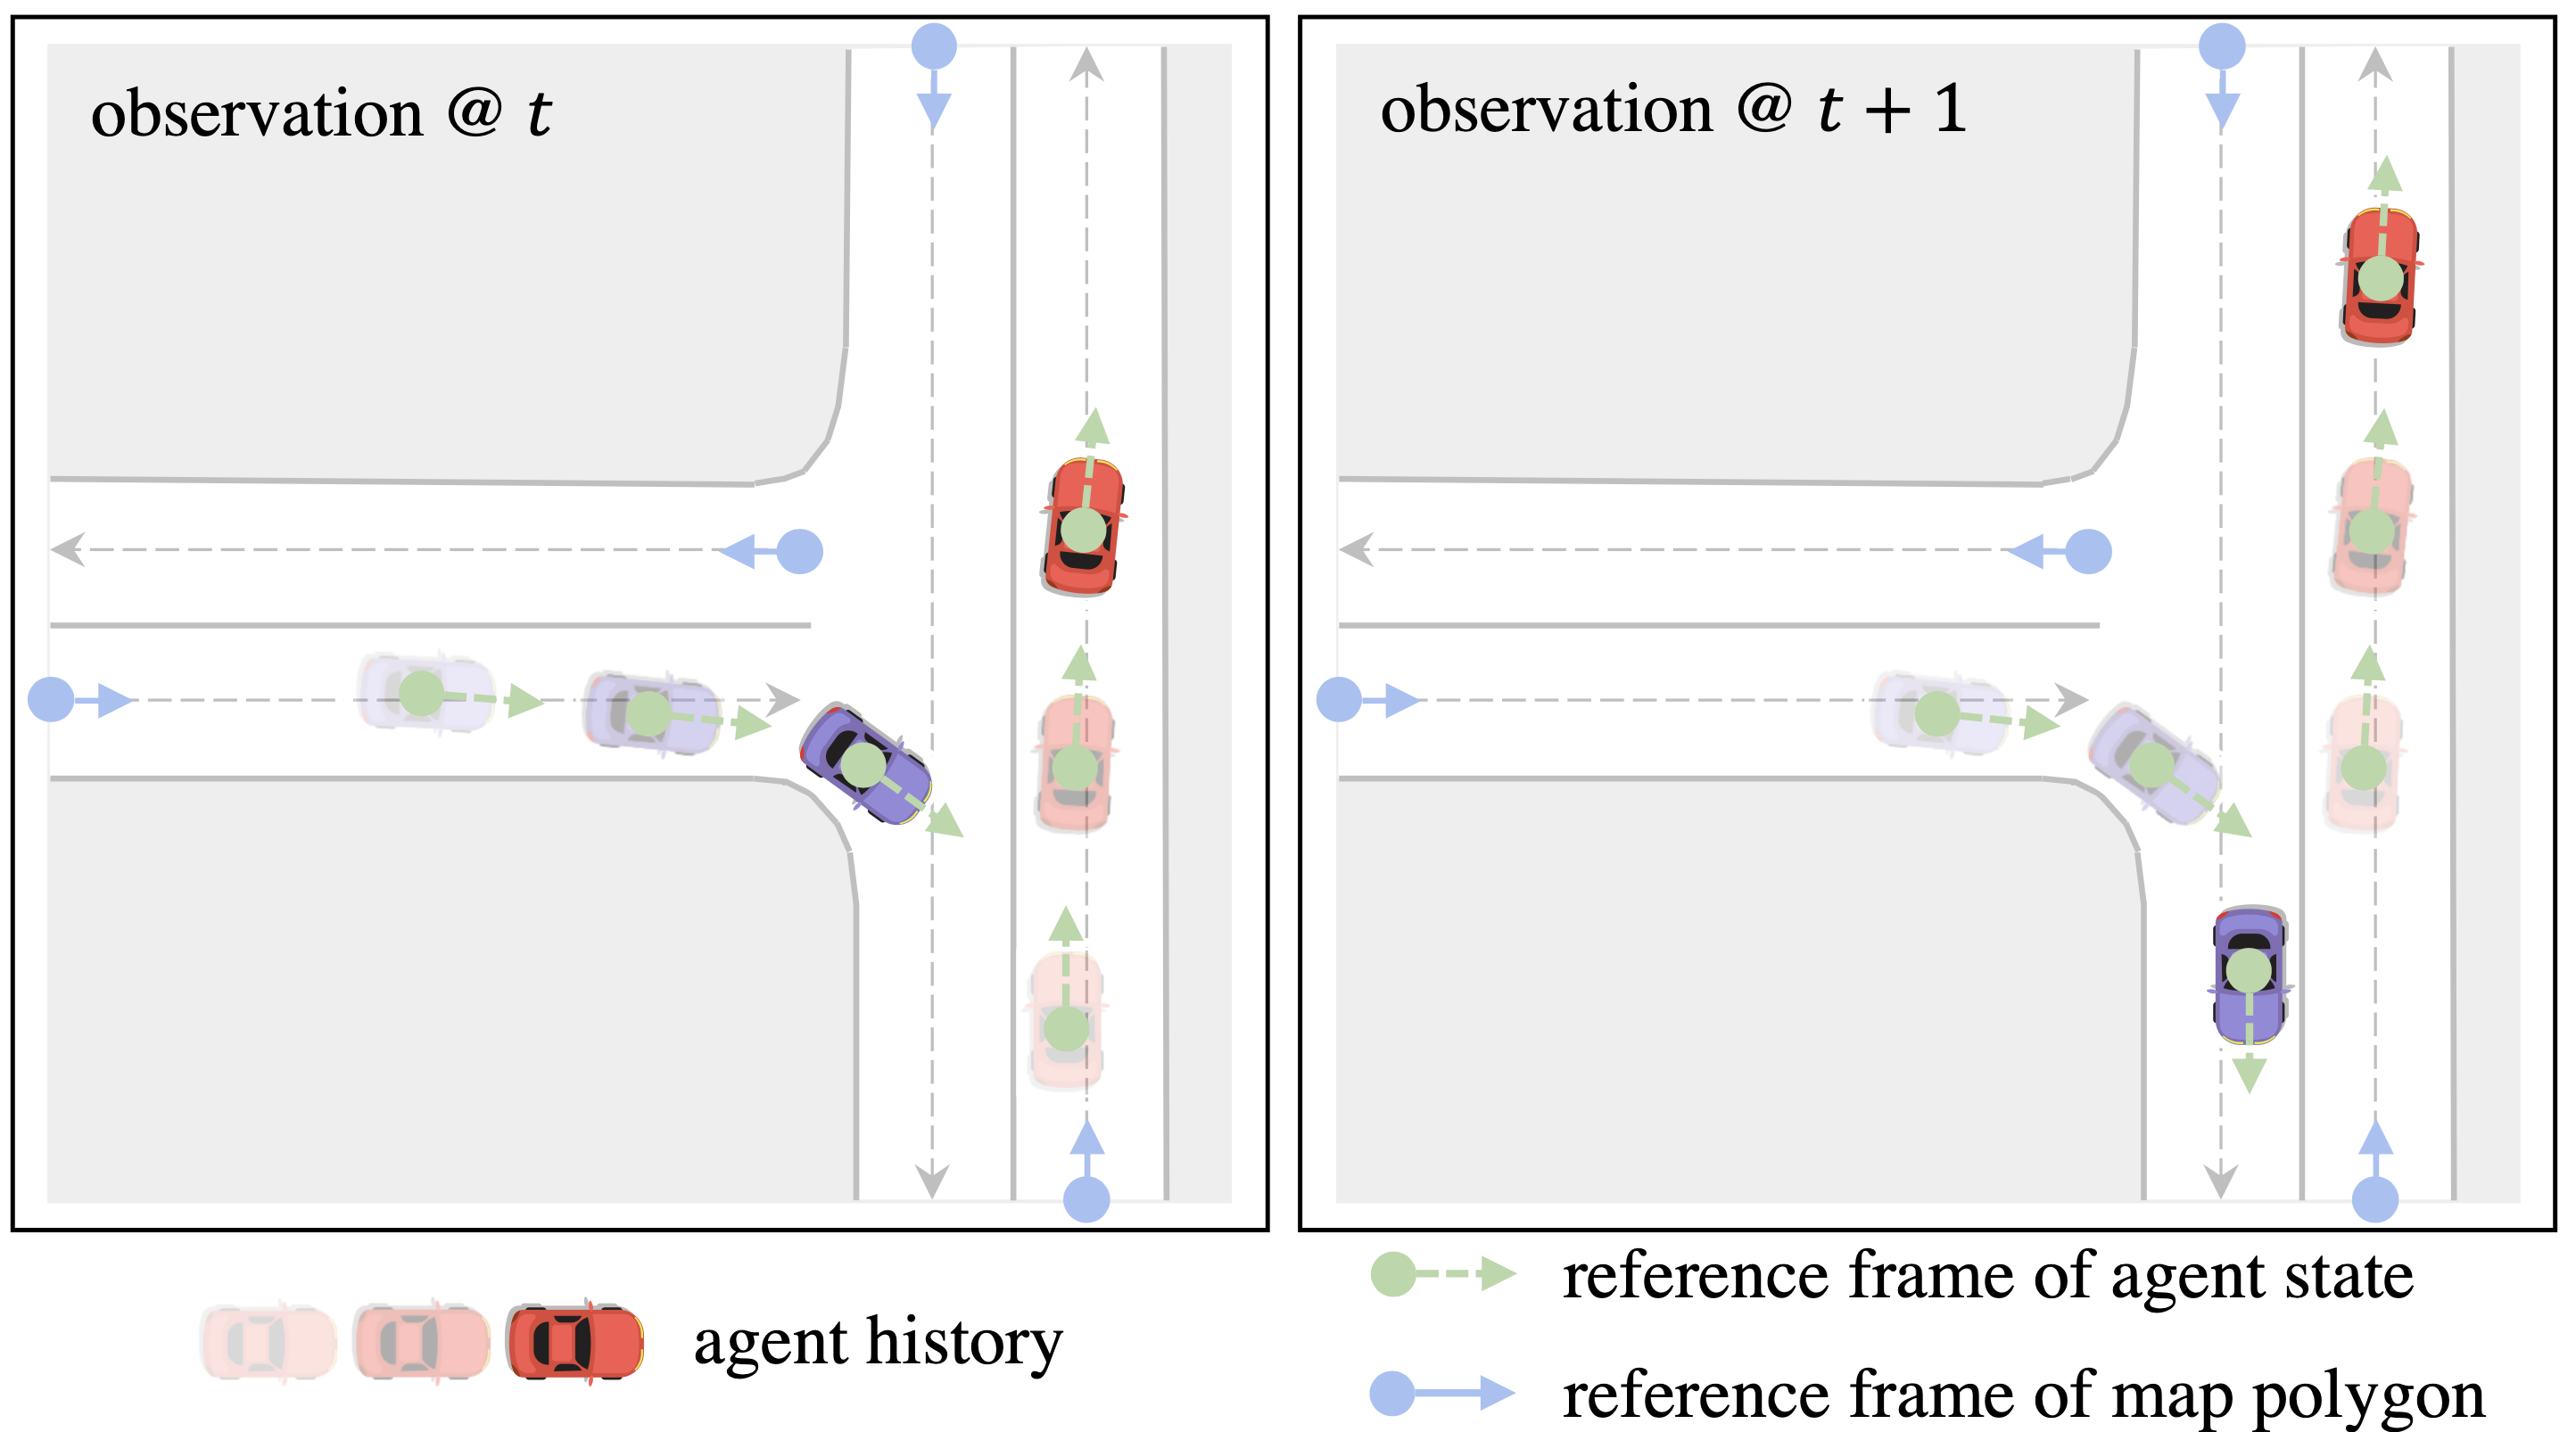
\includegraphics[width=0.5\textwidth]{figures/qc_reference_frame.png}
  \caption{\cite{qcnetZhou2023}~Query-centric encoding: each scene spatio-temporal entity lives in its own local coordinate system}
\end{figure}

Instead of expressing the scene in a single, temporally-evolving global frame, the query-centric paradigm establishes a \emph{local coordinate system} (or \emph{fiber}) for each scene element, in which all spatio-temporal and kinematic properties are expressed. This becomes especially handy, when considering that motion forecasting is inherently a \emph{streaming} task during inference: whenever a new observation arrives, the oldest observation is dropped and the newest one is added to the queue. Hence, two temporally adjacent scene representations share \(T{-}1\) overlapping timesteps, which can be cached and reused in the next step.\\

%% DONE until HERE %%
%%%%%%%%%%%%%%%%%%%%%%%%%%%%%%%%%%%%%%%%%%%%%%%%%%%%%%%%%%%%%%%%%%%%%%%%%%%%%%%%%%%%%%%%%%

\paragraph{A geometric perspective.}

The query-centric paradigm exploits three fundamental symmetries that reflect the underlying physics of trajectory prediction. By placing each scene element (agent or map polygon) in its own local \(\SE{2}\) coordinate frame, this approach dramatically simplifies the learning problem compared to agent-centric methods by theoretically allowing a decomposition of the global scene manifold into a composition of local fibers, each representing a standardized set of spatial and kinematic properties or relatively simple connections between different fibers.

\begin{description}[style=nextline,leftmargin=*]
\item[Permutation invariance.] % TODO: equivariance or invariance?
    Agents and map elements form an unordered set—no element should be  privileged. Query-centric approaches preserve this natural symmetry by treating all elements identically through local frames, while agent-centric methods break symmetry by choosing one agent as the global origin. Formally, for any permutation \(\sigma\) of scene elements, the encoding remains equivariant: \(f(\sigma \cdot S) = \rho(\sigma) f(S)\).

\item[SE(2) invariance.]
    Physical laws are invariant under rigid transformations—translating or rotating the entire scene should not change predictions. For any transformation \(g\in SE(2)\), we require \(f(g\cdot S)=\phi(g)f(S)\) with \(\phi:SE(2)\to GL(d)\) a linear representation. Query-centric encodings achieve this naturally through relative descriptors between local frames, eliminating global coordinate dependence. Agent-centric approaches require explicit re-normalization whenever the reference frame changes, demanding costly re-computation.

\item[Temporal translation invariance.]
    Motion forecasting uses sliding time windows—shifting the time origin should not affect predictions. For any time shift \(\tau\in\mathbb{R}\), the representation satisfies \(f(S(t+\tau))=f(S(t))\). Query-centric methods enable efficient caching since relative temporal descriptors remain unchanged as windows slide. Agent-centric approaches violate this property because their global reference frame evolves with the target agent, requiring full re-encoding at each timestep.
\end{description}

This fiber bundle structure provides the key insight: rather than learning on the high-dimensional manifold of all possible global scene configurations, networks should be able to operate on a factored space where each local fiber encodes standardized spatial and kinematic properties. Since all agents experience similar kinematic constraints and exhibit similar behavioral pattern and all map segments share geometric primitives, the sub-manifolds within individual fibers are remarkably similar across scene elements. This similarity dramatically reduces the required representational capacity—the network primarily learns relationships \emph{between} fibers rather than within them. The relative descriptors connecting all fibers live in a much simpler manifold, further constraining the learning problem. This geometric structure constitutes the key inductive bias distinguishing query-centric from agent-centric paradigms: instead of being forced to model the full complexity of the of global scene variations as a single manifold, the network exploits the underlying symmetries to learn decomposable, fundamentally simpler, more structured representations.


% %%%%%%%%%%%%%%%%%%%%%%%%%%%%%%%%%%%%%%%%%%%%%%%%%%%%%%%%%%%%%%%%%%%%%%%%%%%%%%%%%%%%%%%%%%


% % Furthermore, the entire scene needs to be re-encoded at every timestep as the location and heading of the target agent change
% \paragraph{Local frame construction}
% \begin{description}[style=nextline,leftmargin=*]
%   \item[Agent states.]
%         For agent\(a\) at timestep \(t\) we take the motion vector's \emph{start position} as the origin and align the instantaneous heading with the positive \(x\)-axis\cite{lmformerYadav2025}.
%         The transformation to this frame is
%         \begin{equation}
%             \mathbf x^{(a,t)}_{\text{local}}
%             =\mathbf T_{a,t}^{-1}\,\mathbf x_{\text{global}},
%             \qquad\mathbf T_{a,t}\in SE(2).
%             \label{eq:agent_frame}
%         \end{equation}
%   \item[Map polylines.]
%         Lanes are stored either as \emph{points}
%         \(L_p^i=[P_1^i,\dots,P_K^i]\) or as \emph{segments}
%         \(L_v^i=[V_1^i,\dots,V_{K-1}^i]\) with
%         \(V_k^i=[P_k^i,P_{k+1}^i]\).
%         Each segment's start point acts as the origin and the segment vector defines the \(x\)-axis, leaving only the (normalized) length as an explicit feature.
% \end{description}

% \paragraph{Relative descriptors and embeddings.}
% For any pair \((e_i,t)\), \((e_j,s)\) of scene elements, the query-centric paradigm computes a 4-D descriptor that fully preserves their spatial-temporal offset:
% \[
% r_{j\to i}^{s\to t}=
% \bigl[
%     \|p_j^s-p_i^t\|_2,\;
%     \mathrm{atan2}(p_{j,y}^s-p_{i,y}^t,p_{j,x}^s-p_{i,x}^t)-\theta_i^t,\;
%     \theta_j^s-\theta_i^t,\;
%     s-t
% \bigr].
% \]
% Each component encodes a crucial geometric relationship: \textbf{(i)} The Euclidean distance \(\|p_j^s-p_i^t\|_2\) captures the spatial separation between elements; \textbf{(ii)} The angular offset \(\mathrm{atan2}(\cdot)-\theta_i^t\) represents the bearing from element \(i\) to element \(j\) in \(i\)'s local coordinate frame; \textbf{(iii)} The orientation difference \(\theta_j^s-\theta_i^t\) encodes the relative heading between elements; \textbf{(iv)} The temporal offset \(s-t\) preserves the time relationship between observations.

% This descriptor is embedded via Fourier features and \emph{concatenated} to keys and values inside factorized attention layers. Because both elements live in local frames, \(r_{j\to i}^{s\to t}\) is itself \(SE(2)\)- and time-translation invariant, ensuring the entire representation respects the fundamental symmetries of the physical world.

% \paragraph{Scene element embedding and processing}
% For each spatial-temporal element (agent state or map point), we compute polar coordinates of its geometric attributes (velocity, motion vector, or sampled map-point positions) \emph{relative} to its local frame.
% Each polar tuple is lifted into a high-frequency representation via Fourier features~\cite{qcnetZhou2023}, concatenated with semantic tags (e.g., agent type), and passed through an MLP to yield an embedding.
% For map polygons, we pool their sampled-point embeddings via attention, producing
% \[
% \text{agent embeddings: }[A,T,D],\quad
% \text{map embeddings: }[M,D],
% \]
% where \(D\) is the hidden dimension.
% Since each element's embedding is tied only to its own frame, it can be reused across windows, unlike agent-centric methods that must re-encode everything per agent per step.

% Map polygons undergo self-attention where query from polygon \(i\) attends to neighbors \(\{\mathbf{m}_j\}_{j\in\mathcal N_i}\), with key/value formed by \([\mathbf{m}_j;\mathbf{r}_{j\to i}]\).
% Since all components are query-centric, the output encodings are roto-translation invariant and can be shared across agents or pre-computed offline.

% For agent encoding, factorized attention enables the \(i\)-th agent at time \(t\) to attend: (1)~temporally to past \(\tau\) steps \(\{[\mathbf{a}_i^s;\mathbf{r}_{i\to i}^{s\to t}]\}_{s=t-\tau}^{t-1}\), (2)~spatially to map elements \(\{[\mathbf{m}'_j;\mathbf{r}_{j\to i}]\}_{j\in\mathcal N_i}\), and (3)~socially to neighboring agents \(\{[\mathbf{a}_j^t;\mathbf{r}_{j\to i}^{t\to t}]\}_{j\in\mathcal N_i}\).
% This enables the crucial complexity reduction:
% \[
% \underbrace{\mathcal{O}(AT^2)+\mathcal{O}(ATM)+\mathcal{O}(A^2T)}_{\text{standard factorized attention}}
% \quad\longrightarrow\quad
% \underbrace{\mathcal{O}(AT)+\mathcal{O}(AM)+\mathcal{O}(A^2)}_{\text{query-centric streaming}}.
% \]



% \paragraph{Agent-centric vs.\ query-centric comparison.}

% \begin{description}[style=nextline,leftmargin=*]
%   \item[Computational efficiency and reuse.]
%         Agent-centric: None—recompute full BEV/agent tokens each step (\(O(A T^2)\)); query-centric: Cache and reuse—when the window slides, the \(T-1\) overlapping steps' embeddings are identical and can be reused, reducing cost to \(O(A T)\) and enabling \(<\!10\)ms latency in dense scenes. However, this efficiency comes at a memory cost, as QCNet training consumes approximately 160GB GPU memory~\cite{qcnetZhou2023}.
%         Encodings are independent of prediction target and can be shared across agents and time steps.
%   \item[Symmetry preservation and multi-agent reasoning.]
%         Agent-centric breaks permutation symmetry by privileging one agent; query-centric treats all elements equally, preserving the natural symmetry among multiple agents and enabling true joint prediction rather than marginal approaches.
%         Parallel decoding: Usually one-agent-at-a-time for agent-centric; multi-agent parallel with the same invariant scene tensor shared by all target agents for query-centric.
%   \item[Streaming and invariance properties.]
%         Query-centric caches invariant tensors across sliding windows and supports parallel prediction for all agents using the same scene encoding; agent-centric re-normalizes each step and requires separate encodings per agent.
%         Latent scene representations are \(SE(2) \rtimes \R\) invariant through the relative descriptors.
%   \item[Memory vs.\ computation trade-off.]
%         QCNet's tensors are shared by all targets but grow linearly with scene size; large-scene training can hit GPU limits.
%         Agent-centric stores fewer per-element relations but recomputes them repeatedly.
%   \item[Inductive bias and learning efficiency.]
%         Efficient reuse: Encodings are independent of prediction target and can be shared across agents and time steps.
%         Local fibres (all isomorphic to \(SE(2)\)) mean the network only learns relations \emph{between} fibres; the sub-manifold to model is smaller, requiring less representational capacity~\cite{bronstein2017geometric}.
%         This dramatically shrinks the global manifold of possible scene encodings compared to agent-centric approaches.
%         Joint prediction capability: Unlike marginal prediction approaches, query-centric models can effectively capture future social interactions among agents.
% \end{description}

% \paragraph{Take-away.}
% By framing scene elements as fibres over \(SE(2)\) and encoding only \emph{relative} pose/time, query-centric representations furnish strong geometric inductive biases, enable massive computation reuse, and support truly parallel multi-agent decoding. These qualities underlie QCNet~\cite{qcnetZhou2023}, LMFormer~\cite{lmformerYadav2025}, and related trajectory prediction models that leverage this paradigm.